\documentclass[a4paper, 12pt]{article}

\usepackage{cmap}
\usepackage{mathtext} 
\usepackage[T2A]{fontenc}
\usepackage[utf8]{inputenc}
\usepackage[english,russian]{babel}	

\usepackage{amsfonts,amssymb,amsthm,mathtools}
\usepackage{amsmath}
\usepackage{icomma} 

\usepackage{graphicx} 
\graphicspath{{Picturies/}}
\usepackage{wrapfig}

\usepackage{array,tabularx,tabulary,booktabs}
\usepackage{longtable}
\usepackage{multirow}

\usepackage{caption}
\captionsetup{labelsep=period}

\renewcommand{\phi}{\varphi}
\newcommand{\eps}{\varepsilon}
\renewcommand{\AA}{\ensuremath{\mathring{A}}}
\newcommand{\parag}[1]{\paragraph*{#1:}}

\newcounter{Points}
\setcounter{Points}{1}
\newcommand{\point}{\arabic{Points}. \addtocounter{Points}{1}}

\author{Вязовцев Андрей, Б01-005}
\date{17.09.22}
\title{Лабораторная работа 5.5.1. Измерение коэффициента ослабления потока $\gamma$-лучей в веществе и определение их энергии.}

\begin {document}

\maketitle

\parag {Цель работы} определение средней энергии $\gamma$-квантов источника.

\parag {В работе используются} сцинтилляционный счётчик; образцы свинца, железа и аллюминия; источник $\gamma$-квантов.

\parag {Теоретическая справка} ~\\

Гамма-лучи возникают при переходе возбуждённых ядер из одного энергетического состояния в другое, более низкое. Эти кванты не имеют ни заряда, ни массы. При прохождении через вещество, пучок квантов будет рассеиваться, а интенсивность уменьшаться по экспоненциальному закону, который можно записать в двух эквивалентных формах:

\begin{align}
    I &= I_0 e^{-\mu l}  \label{eq:int} \\ 
    I &= I_0 e^{-\mu^\prime m_1}
\end{align}

При прохождении через вещество $\gamma$-кванты испытывают рассеяние по нескольки причинам:

\begin{enumerate}
    \item Фотоэлектрическое поглащение. Этот процесс, по-сути, является обратным к процессу испукания квантов, описанному выше: $\gamma$-кванты сталкиваются с электронами внутренних оболочек, после чего электроны поглощают кванты, переходя на более высокий энергетический уровень.
    \item Комптоновское рассеянияние. В этом случае кванты сталкиваются со свободными электронами. В результате этого электрон приобретает энергию, а квант, наоборот, --- теряет (и, соответственно, частота кванта уменьшается).
    \item Образование пар. Согласно интерпретации Дирака, электроны с отрицательными энергиями создают равномерный, ненаблюдаемый фон. Но $\gamma$-квант может столкнуться с таким электроном в электрическом поле ядер (для этого его энергия должна быть больше $2mc^2$), после чего образуется электрон-позитронная пара.
\end{enumerate}

Полный линейный коэффициент $\mu$ ослабления пучка $\gamma$-квантов при прохождении через вещество равен сумме коэффициентов для всех трёх процессов. В хорошей геометрии (когда все рассеянные $\gamma$-кванты не попадают на счётчик) количество рассеянных частиц пропорционально их общему количеству и длине пути, т.е.

\[
    -dN = \mu N dl
\]

Отсюда получается формула, аналогичная \eqref{eq:int}:

\begin{equation}
    N = N_0 e^{-\mu l}
    \label{eq:num}
\end{equation}

\parag {Экспериментальная установка} ~

На рис. \ref{pic:work1} блок-схема установки, используемой для измерения коэффициентов ослабления потока $\gamma$-лучей. На нём:

\begin{itemize}
    \item И --- источник $\gamma$-лучей
    \item Pb --- свинцовый контейнер с коллиматорным каналом
    \item П --- набор поглотителей
    \item С --- сцинтиллятор (кристалл NaI (Tl))
    \item Ф --- усилитель-формирователь
\end{itemize}

\begin{figure}[!h]
    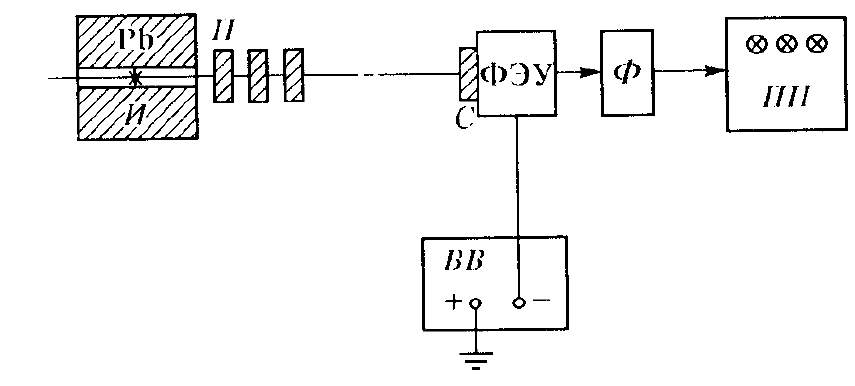
\includegraphics[scale = 0.4]{Workplace1}
    \centering
    \caption{Блок-схема установки, используемой для измерения коэффициентов ослабления потока $\gamma$-лучей.}
    \label{pic:work1}
\end{figure}

На рис. \ref{pic:work2} изображена схема поглощения $\gamma$-квантов.

\begin{figure}[!h]
    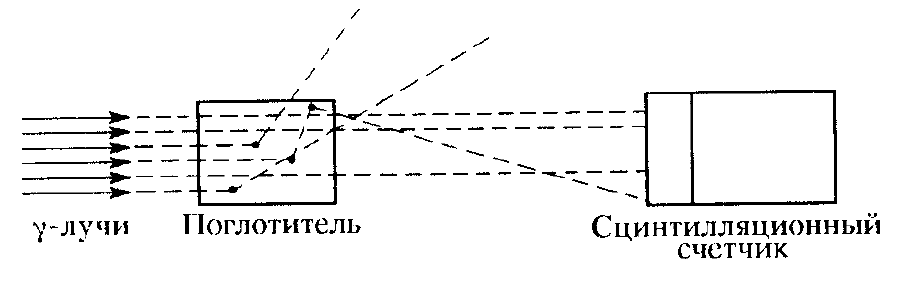
\includegraphics[scale = 0.4]{Workplace2}
    \centering
    \caption{Схема рассеяния $\gamma$-квантов в поглотителе.}
    \label{pic:work2}
\end{figure}

\parag {Ход работы} ~\\

\point Включим приборы, дадим им прогреться 5---10 минут.

\point Убедимся, что установка <<чувствует>> $\gamma$-лучи. Для этого включим счётчик и будем убирать и ставить свинцовую пробку. При этом скорость изменения показаний должна резко увеличиваться и падать соответственно.

\point Теперь перейдём к изучению поглощения лучей в свинце, железе и алюминии. Для этого будем ставить образец какого-то материала, измерять количество частиц, пролетающих через него за определённое время, потом добавлять ещё один образец и т.д. до десяти штук. Измерять будем всегда до $40000$ $\gamma$-лучей или $200$ секунд. Также будем замерять размер каждого образца с помощью штангенциркуля. Результаты измерений представлены в таблицах \ref{tab:1}, \ref{tab:2} и \ref{tab:3}.

% Требование относительно 40000 или 200 --- от моего лабника, Аникина (F)

\point Теперь измерим фон, который обусловлен шумом счётчика и посторонними частицами. Для этого закроем источник свинцовой пробкой, после чего запустим счётчик. Получаем:

\begin{align*}
    N_0 &= 4102 \\
    t_o &= 300~c
\end{align*}

\parag {Обработка результатов} ~\\

\point В формуле \eqref{eq:num} для того, чтобы учесть фон, следует перейти перейти от количества частиц к их количеству за единицу времени, т.е. от $N$ к $\dfrac{N}{t}$. Тогда $\dfrac{N}{t} - \dfrac{N_0}{t_0}$ --- <<чистое>> количество частиц. Т.~к. наша задача --- найти коэффициент $\mu$, то следует использовать логарифмическую шкалу. Итак, построим графики: $\ln (\dfrac{N}{t} - \dfrac{N_0}{t_0}) (l)$.

Исходя из наклонов графиков, получаем:

\begin{align*}
    \mu_{Al} &= (0.203 \pm 0.006) ~ см^{-1} \\
    \mu_{Pb} &= (1.156 \pm 0.018) ~ см^{-1} \\
    \mu_{Fe} &= (0.581 \pm 0.006) ~ см^{-1} 
\end{align*}

Здесь учитываются только ошибка МНК, но стоит также учесть ошибку счётчика, таймера и штангенциркуля. Погрешность первого мы попытались <<устранить>> путём учёта фона, оценить её не представляется возможным. Второй проводил измерения с точностью $0.01$ с, что пренебрежимо мало с наименьшим измерением в $10$ с. Погрешность последнего --- $0.1$ мм, что даёт погрешности от $0.5\%$ до $2\%$. Итого получаем:

\begin{align*}
    \mu_{Al} &= (0.203 \pm 0.006) ~ см^{-1} \\
    \mu_{Pb} &= (1.16  \pm 0.03)  ~ см^{-1} \\
    \mu_{Fe} &= (0.581 \pm 0.008) ~ см^{-1}
\end{align*}

Из изображения \ref{img:energy} можно найти среднюю энергию $\gamma$-квантов. Получаем:

\begin{align*}
    E_{Al} &= (0.6 \div 0.7) ~ МэВ \\
    E_{Pb} &= (0.6 \div 0.8) ~ МэВ \\
    E_{Fe} &= (0.6 \div 0.7) ~ МэВ
\end{align*}

Из источника, очевидно, во время разных экспериментов вылетали схожие кванты. Следовательно, схожесть энергий подтверждает верность эксперимента.

\parag {Приложение. Tаблицы и графики} ~\\

\begin{table}[!h]
    \centering
    \begin{tabular}{|c|c|c|c|c|c|c|c|c|c|c|}
        \hline
        № & 1 & 2 & 3 & 4 & 5 & 6 & 7 & 8 & 9 & 10\\ \hline
        $l_{обр}$, мм & 20.0 & 20.3 & 20.1 & 19.9 & 19.7 & 20.1 & 20.0 & 20.2 & 19.8 & 19.7\\ \hline
        $l_{общ}$, мм & 20.0 & 40.3 & 60.4 & 80.3 & 100.0 & 120.1 & 140.1 & 160.3 & 180.1 & 199.8\\ \hline
        N & 46000 & 64000 & 40000 & 52501 & 43112 & 46125 & 58800 & 53099 & 36662 & 25475\\ \hline
        t, с & 10 & 20 & 20 & 40 & 50 & 80 & 100 & 200 & 200 & 200
        \\ \hline
    \end{tabular}
    \caption {Алюминий.}
    \label{tab:1}
\end{table}

\begin{table}[!h]
    \centering
    \begin{tabular}{|c|c|c|c|c|c|c|c|c|c|c|}
        \hline
        № & 1 & 2 & 3 & 4 & 5 & 6 & 7 & 8 & 9 & 10\\ \hline
        $l_{обр}$, мм & 5.0 & 5.0 & 5.0 & 4.7 & 4.6 & 5.0 & 4.4 & 4.8 & 5.1 & 4.9\\ \hline
        $l_{общ}$, мм & 5.0 & 10.0 & 15.0 & 19.7 & 24.3 & 29.3 & 33.7 & 38.5 & 43.6 & 48.5\\ \hline
        N & 43041 & 44128 & 47372 & 52100 & 76190 & 43330 & 29139 & 18184 & 11616 & 8314\\ \hline
        t, с & 10 & 20 & 40 & 80 & 200 & 200 & 200 & 200 & 200 & 200
        \\ \hline
    \end{tabular}
    \caption {Свинец.}
    \label{tab:2}
\end{table}

\begin{table}[!h]
    \centering
    \begin{tabular}{|c|c|c|c|c|c|c|c|c|c|c|}
        \hline
        № & 1 & 2 & 3 & 4 & 5 & 6 & 7 & 8 & 9 & 10\\ \hline
        $l_{обр}$, мм & 10.1 & 10.2 & 10.1 & 10.3 & 10.0 & 10.0 & 10.1 & 10.1 & 10.0 & 10.1\\ \hline
        $l_{общ}$, мм & 10.1 & 20.3 & 30.4 & 40.7 & 50.7 & 60.7 & 70.8 & 80.9 & 90.9 & 101\\ \hline
        N & 46770 & 47883 & 51174 & 41074 & 77237 & 44965 & 26906 & 16397 & 10624 & 7340\\ \hline
        t, с & 10 & 20 & 40 & 60 & 200 & 200 & 200 & 200 & 200 & 200
        \\ \hline
    \end{tabular}
    \caption {Железо.}
    \label{tab:3}
\end{table}

\begin{figure}[!h]
    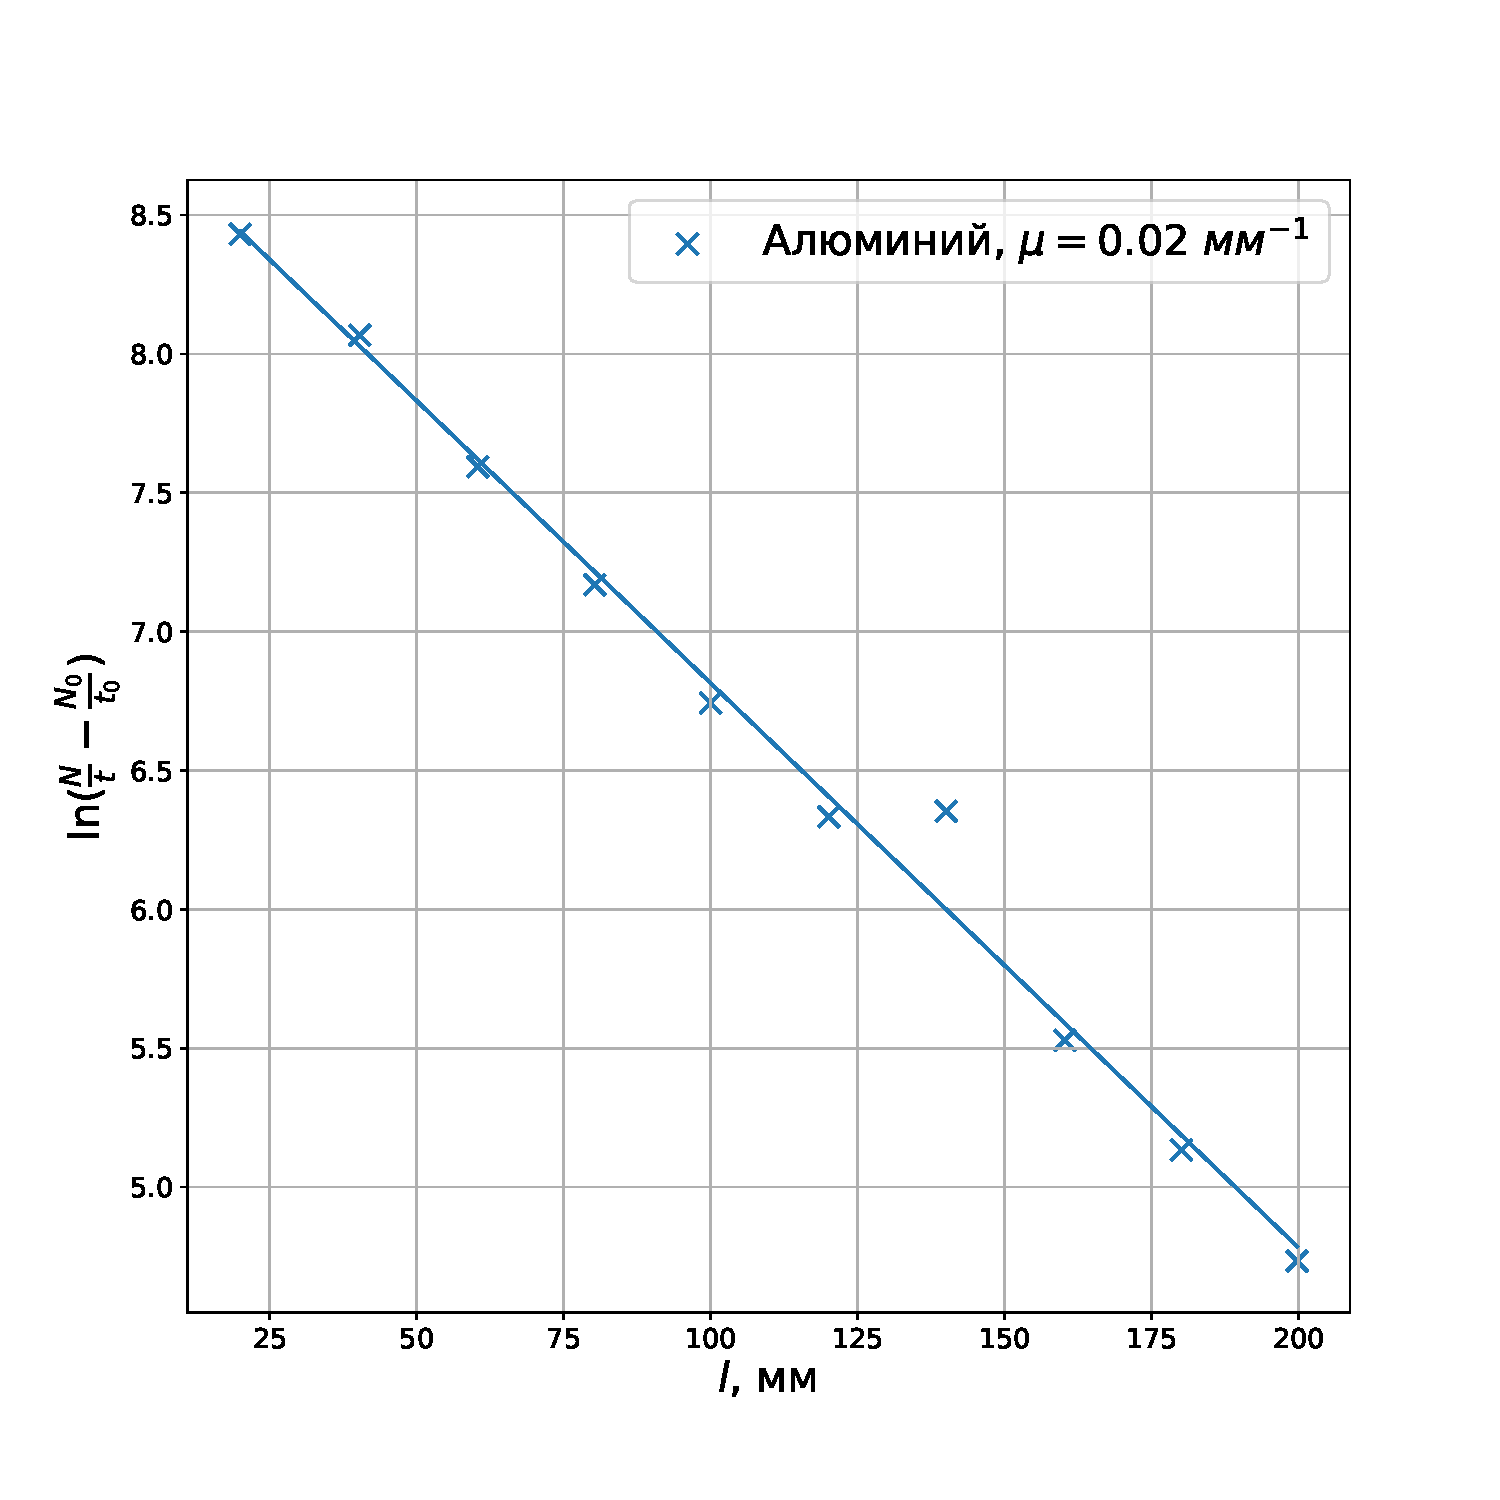
\includegraphics[scale = 0.35]{graph0}
    \centering
    \caption{Алюминий, $\ln (\dfrac{N}{t} - \dfrac{N_0}{t_0}) (l)$}
\end{figure}

\begin{figure}[!h]
    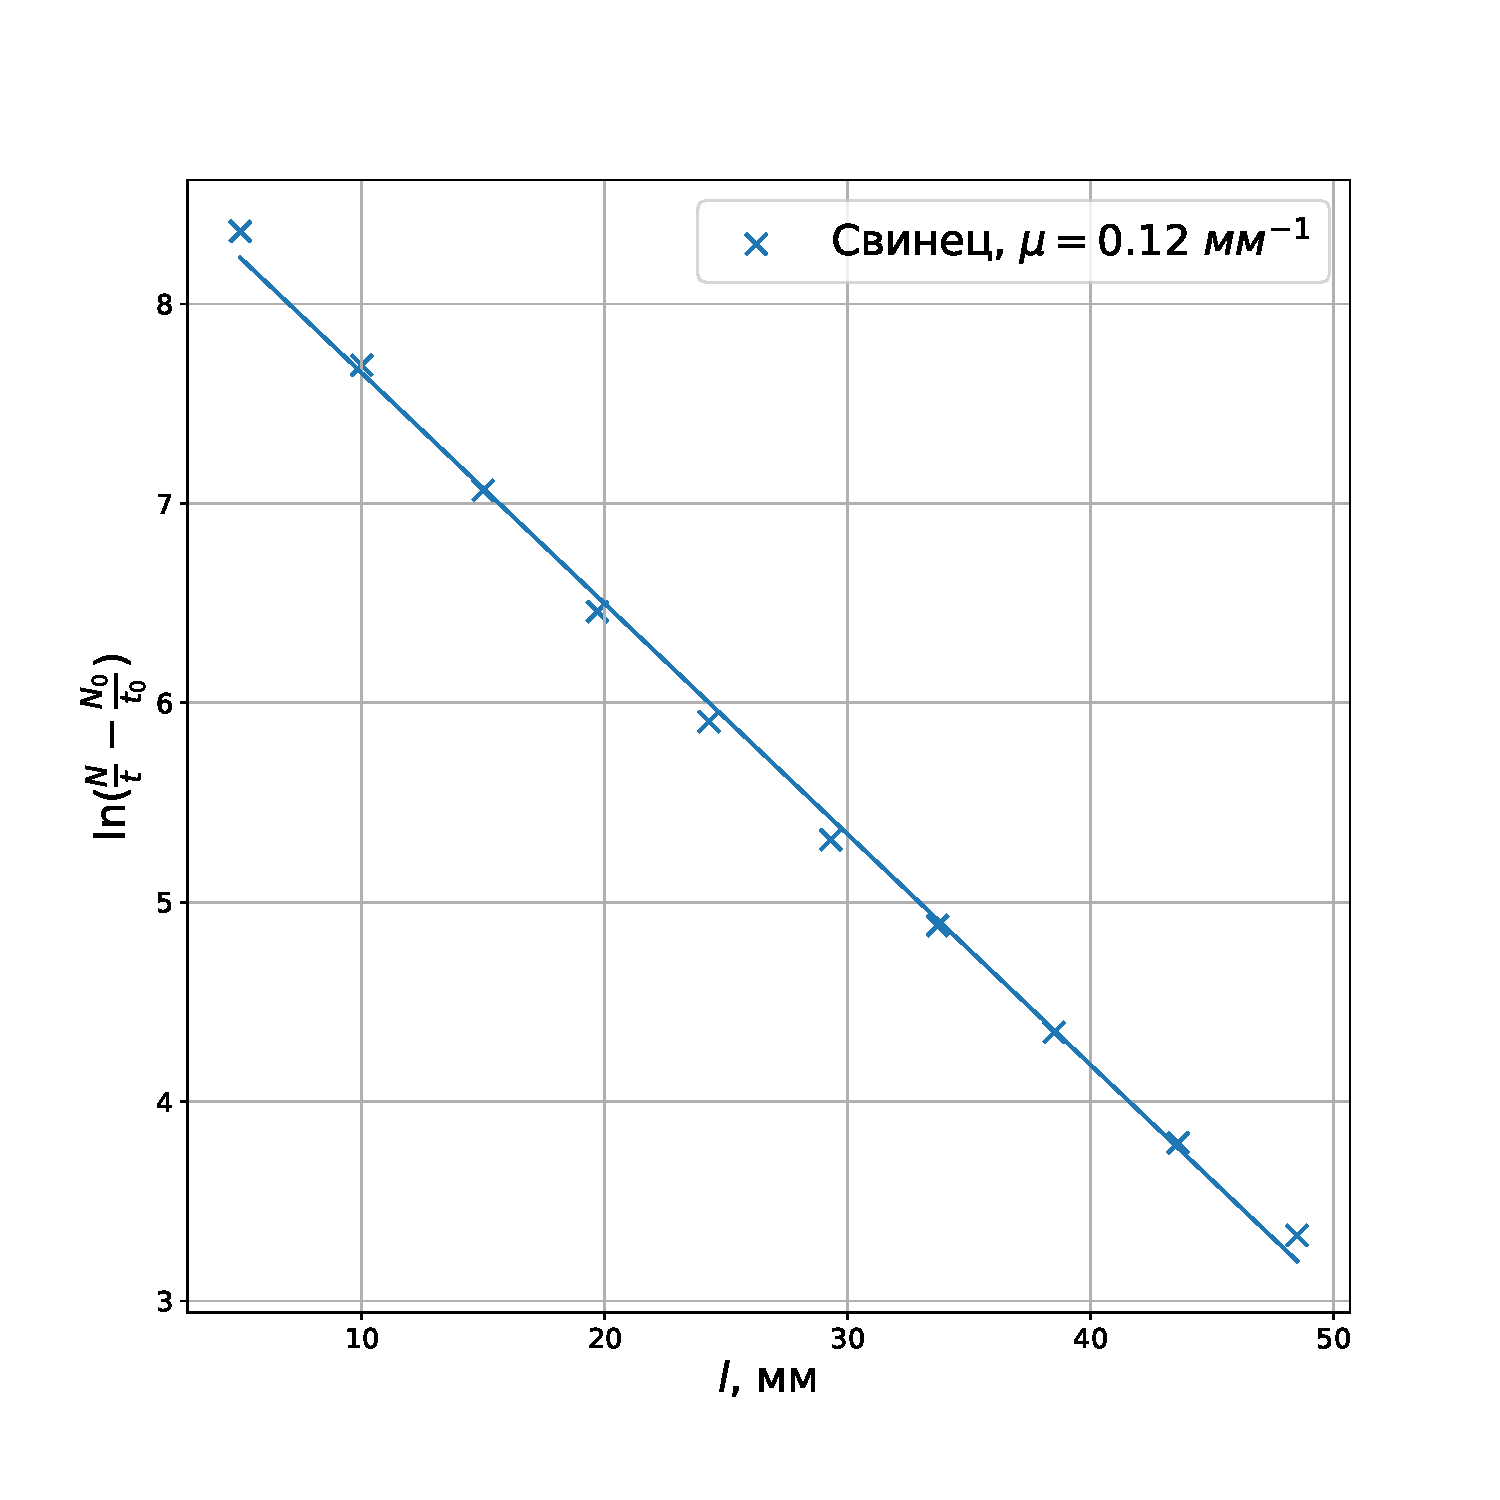
\includegraphics[scale = 0.35]{graph1}
    \centering
    \caption{Свинец, $\ln (\dfrac{N}{t} - \dfrac{N_0}{t_0}) (l)$}
\end{figure}

\begin{figure}[!h]
    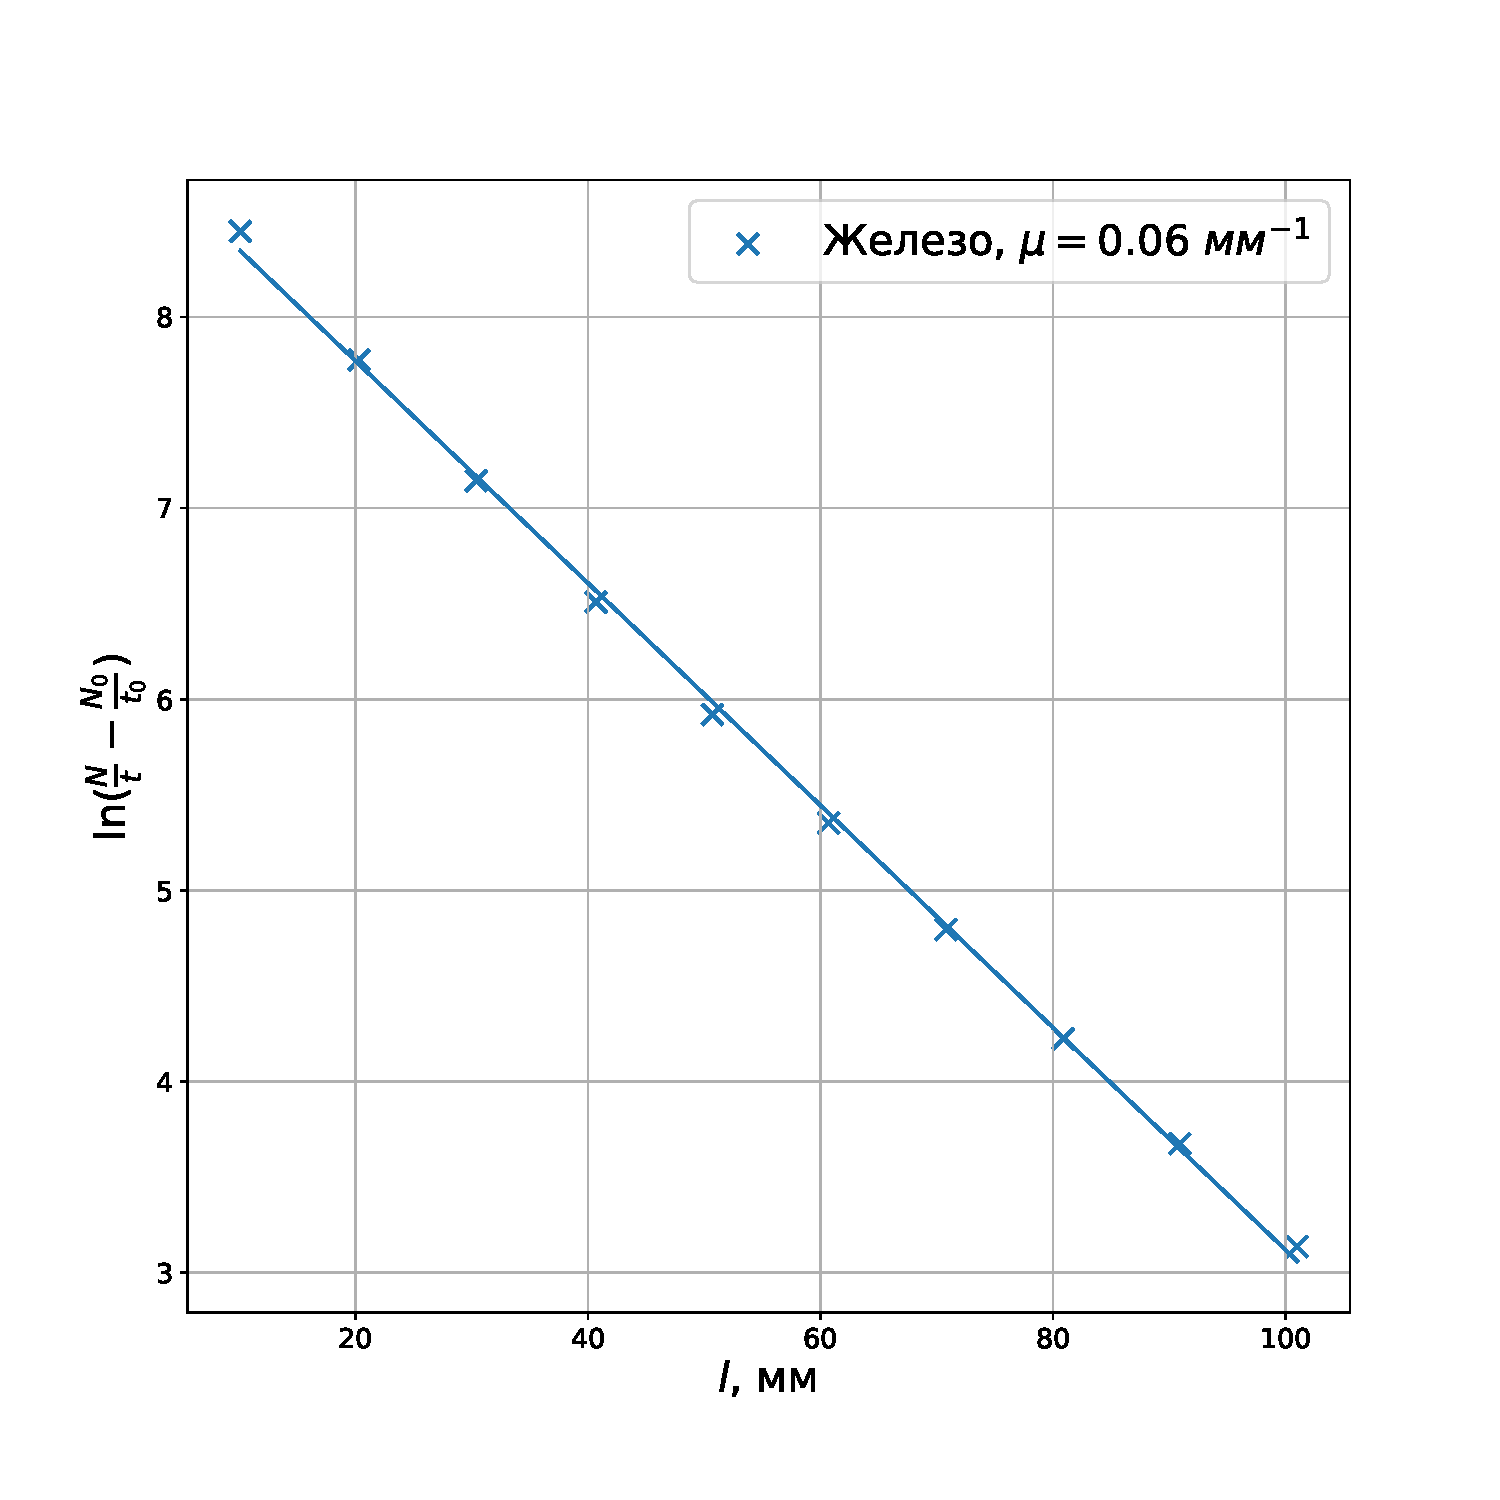
\includegraphics[scale = 0.35]{graph2}
    \centering
    \caption{Железо, $\ln (\dfrac{N}{t} - \dfrac{N_0}{t_0}) (l)$}
\end{figure}

\begin{figure}[!h]
    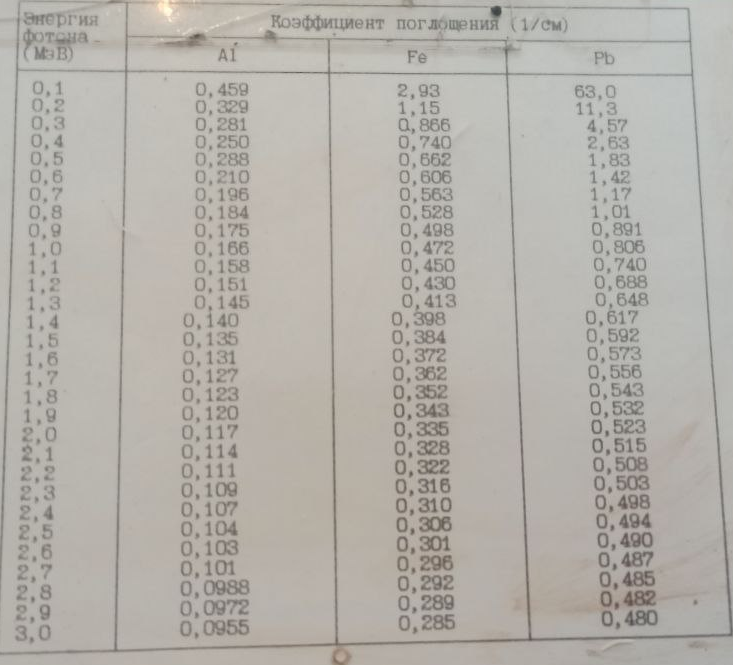
\includegraphics[scale = 1.2]{energy}
    \centering
    \caption{Табличные данные}
    \label{img:energy}
\end{figure}

\end {document}
